\section{Lastenheft}
In diesem Kapitel wird das Lastenheft erläutert. Es wird erläutert, wie die Lasten bestimmt wurden

Damit die Erklärung des Lastenheftes und der gesammte Auslegungsprozess an sich verständlicher wird, werden zuerst die verwendeten Begriffe definiert.\\
Als \emph{Modus} wird ein ''Zustand`` oder eine ''Position`` des Solar Butterflys verstanden. Modus \emph{A} beschreibt zum Beispiel den Solar Butterfly im ''Fahr-Modus``. In diesem Fall würde dies bedeuten, dass alle Panelen, Stützen und Seitenmodule eingefahren sind. Es wird für jeden der vier definierten Modi ein FEM-Modell erstellt.\\
Als \emph{Lastfall} wird eine Situation (z.B. Fahrt auf einer um 10° geneigten Strasse) oder eine Last (z.B. Personenlast) verstanden, welche in einem spezifischen Modus auftreten kann. Der Lastfall \emph{1.1} im Modus \emph{A} beschreibt zum Beispiel die vertikale Beschleunigung von 1.25 g welche durch das Überfahren einer Bresmmschwelle auftreten kann. Der Lastfall \emph{1.1} im Modus \emph{C} beschreibt eine Personenlast. Ein Lastfall ist vollständig definiert, wenn klar ist, wie dieser im jeweiligen FEM-Modell des betreffenden Modus, einzugliedern ist.\\
Der Lastfall \emph{1.1} im Modus \emph{A} ist nicht notwendigerweise der Selbe, wie der Lastfall \emph{1.1} im Modus \emph{B} oder \emph{C}! Die klare Zuweisung der Lastfälle zu einem spezifischen Modus wurde vorgenommen, um die Anzahl der Lastfälle in den verschiedenen Modi gering zu halten und die daraus resultierenden Lastkombinationen pro Modus übersichtlicher zu gestalten. Dies führt mit sich, da gewisse Lastfälle in mehreren Modi vorkommen, dass einige Lastfälle doppelt aufgeführt werden. So wird zum Beispiel der Lastfall \emph{Neigung Stehend} im Modus \emph{B} und \emph{C} aufgeführt, da die Situation des geneigten Bodens im parkierten Zustand in beiden Modi auftreten kann. Alle Lastfälle welche in diesen Modi nicht auftreten, können jedoch weggelassen werden, wodurch - wie bereits erwähnt - das Lastenheft übersichtlicher gestaltet werden kann.\\
Als \emph{Lastkombination} wird eine Kombination von verschiedenen Lastfällen verstanden. Eine Lastkombination bezieht sich jeweils auf einen Modus. Die Lastkombination A.3.1.2.1 setzt sich zusammen aus dem Modus \emph{A} und den Lastfällen 1.3, 2.1 3.2 und 4.1 aus dem Modus \emph{A}.

Folgend werden die vier Modi mit den dazugehörigen Lastfällen vorgestellt. Es wird jeweils beschrieben, wie die Lasten zustande kommen und wie diese in den FEM-Modellen eingebunden werden.

\subsection{Modus A: Fahren}
Der Modus \emph{A} beschreibt den Solar Butterfly im ''Fahr-Modus`` und ist in der Abbildung \ref{Modus A} dargestellt. Konkret bedeutet dies, dass alle Panelen und Seitenmodule eingefahren und über die Verschlüsse fest mit dem Rest des Aufbaus verbunden sind. Ebenfalls sind die alle Stützen eingefahren. Im Fahr-Modus befinden sich keine Personen im Solar Butterfly und das Mobiliar ist an den dafür vorgesehenen Stellen verstaut. Weiter herrscht in allen Lastkombinationen die Erdbeschleunigung von 1 g. Der Lastfall von 1 g wird nicht spezifisch aufgeführt.

\begin{center}
  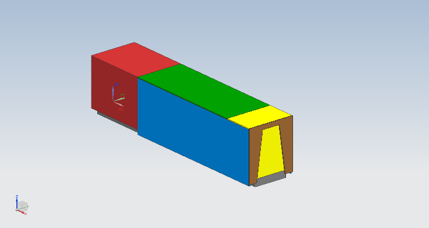
\includegraphics[width=0.5\textwidth]{04_Figures/A.png}
  \captionof{figure}{Modus A}
  \label{Modus A}
\end{center}

  \paragraph{Beschleunigungen durch Fahren}
  \begin{description}
    \item \textbf{1.1 Vertikale Beschleunigung}\\
    Zusätzlich zur vertikalen Beschleunigung durch die Erdanziehung, entstehen durch das Überfahren von Schlaglöcher und Bremsschwellen vertikale Beschleunigungen.\\
    In einem ersten Ansatz wurde der Solar Butterfly als ein \emph{Ein-Massen-Schwinger}-System modelliert und die Beschleunigung beim Überfahren einer Sinusförmigen Bremsschwelle numerisch ermittelt.\\

    Die Position des Rades während dem Überfahren der Bremsschwelle ist gegeben durch folgenden Zusammenhang:
    \begin{equation}
      x_r^n = h \cdot sin\left(\pi \cdot \frac{n\Delta t \cdot v}{l}\right)
    \end{equation}
    $l$ steht dabei für die Länge, und h für die Höhe der Bremsschwelle.\\

    Um die Beschleunigung des Solar Butterflys zu berechnen, wird in einem ersten Schritt dessen Position zum Zeitpunk $n$ $x_{SB}^n$ aus der vorangehenden Situation berechnet.
    \begin{equation}
      x_{SB}^n = x_{SB}^{(n-1)} + v^{(n-1)} \cdot \Delta t
    \end{equation}

    Als nächstes wird der Federweg $s^n$, sowie die Änderungsrate des Federwegs $v_s^n$ zum Zeitpunkt $n$ aus den Positionen des Rades $r_x^n$ und des Solar Butterflys $x_{SB}^n$ berechnet.
    \begin{equation}
      s^n = x_r^n - x_{SB}^n
    \end{equation}
    \begin{equation}
      v_s^n = \frac{s^n - s^{(n-1)}}{\Delta t}
    \end{equation}

    Die Beschleunigung des Solar Butterfly ergibt sich dann zu:\\
    \begin{equation}
      a_{SB}^n = \frac{k \cdot s^n + d \cdot v_s^n}{m}
    \end{equation}

    Wobei $k$ für die Federkonstante und $d$ für die Dämpfungskonstante stehen.
    Die aus der Beschleunigung des Solar Butterfly resultierende neue Geschwindigkeit, kann wie folgt berechnet werden.
    \begin{equation}
      v^n = v^{(n-1)} + a_{SB}^n \cdot \Delta t
    \end{equation}

    Das \emph{Ein-Massen-Schwinger}-Modell wurde mit einer Masse von 2200 kg, einer mittleren Federkonstante, gegeben aus den Datenblättern des Herstellers [ANHANG], von 353'000 N/m und einer Dämpfungskonstante von 3500 Ns/m modelliert. Beim Überfahren einer Bremsschwelle von 0.9 m Länge und 0.1 m Höhe mit einer Geschwindigkeit von 40 km/h resultiert eine maximale Beschleunigung von rund 1.6 g. Die Berechnung ist im [Elektronischen Anhang] zu finden.\\
    Zu der Berechnung muss gesagt werden, dass es sich um ein eher konservatives Modell handelt und die erhaltene Beschleunigung zu hoch liegt. So wurde zum Beispiel die Federung durch die Reifen nicht berücksichtigt. Weiter befindet sich der Massenschwerpunkt nicht in der Federachse, was eine weitere Abminderung der Beschleunigung zur folge hat.\\

    Um die zu wählende Beschleunigung breiter abstützen zu können, wurden andere Arbeiten zum Thema herbeigeführt. \emph{Janczur} \cite{Beschl.1} zeigt, dass beim Überfahrein einer Bremsschwelle von 0.36 m Länge und einer Höhe von 0.05 m, mit einer Geschwindigkeit von 40 km/h, in der Fahrzeugmitte eines Personenwagens, Beschleunigungen von 0.71 g herrschen. Direkt über der Fahrzeugachse treten Beschleunigungen von bis zu 1.5 g auf.\\
    \emph{García-Pozuelo} et al. \cite{Beschl.2} massen in der Fahrzeugmitte eines Personenwagens Beschleunigungen von 0.73 g beim Überfahrein einer Bremsschwelle von 0.9 m Länge und 0.1 m Höhe. Dies bei einer Geschwindigkeit von 50 km/h.\\
    \emph{Haniszewski} et al. \cite{Beschl.3} massen Beschleunigungen, welche eine Person auf der Rückfahrbank eines Personenwagens während dem Überfahren einer Bremsschwelle erfährt. Sie massen Beschleunigungen von bis zu 1 g. Direkt über der Fahrzeugachse wurden Beschleunigungen von 1.3 g gemessen. Dies bei einer Geschwindigkeit von 30 km/h und einer Bremsschwelle von 0.5 m Länge und 0.05 m Höhe.\\
    \emph{Pidl} \cite{Beschl.4} zeigt, dass Transportware in einem Sattelschlepper Beschleunigungen von +- 1 g erfahren. Ob diese maximal gemessene Beschleunigung beim Überfahren einer Bremsschwelle erreicht wurde, ist nicht ersichtlich.

    Es wird davon ausgegangen, dass
    Ähnliche Beschleunigungen wie PKW
    jedoch Tiefere Geschwindigkeiten da zu erst Zugfahrzeug über die Schwelle fährt.
    daher wieder tiefer

    Schluss: 1.25g vertikale Beschleunigung

    \item \textbf{1.2 Longitudinale Beschleunigung}\\
    Longitudinale positive Beschleunigungen in Fahrtrichtung entstehen durch eine Erhöhung der Fahrgeschwindigkeit durch das Zugfahrzeug. Das \emph{Institut für Unfallanalysen Hamburg} \cite{Verz.3} benützt die Beschleunigung von Personenwagen von maximal 0.3g und von Lastkraftwagen von 0.1 g, als Anhaltswerte. \\

    Longitudinale Verögerungen entstehen durch abminderung der Fahrgeschwindigkeit. Die extremste graduelle Verzögerung entsteht dabei durch eine Notbremsung.\\
    \emph{Kudarauskas} \cite{Verz.1} zeigt bei seiner Analyse der Notbremsungen von Personenwagen, dass die maximale Verzögerung bei rund 0.9 g liegt. Das \emph{Institut für Unfallanalysen Hamburg} \cite{Verz.2} zeiht bei Gutachten die Vollverzögerung von 0.8 g für Personenwagen und 0.7 g für Lastkraftwagen als standard Werte herbei. \\

    Longitudinale Beschleunigungen durch Unfälle werden gekonnt verdrängt.

    Schluss: +0.2 -0.8g

    \item \textbf{1.3 Laterale Beschleunigung}\\
    Laterale Beschleunigungen entstehen hauptsächlich beim Kurvenfahren und sind abhängig von der Geschwindigkeit mit welcher die Kurve durchfahren wird und des Kurvenradius.\\
    \emph{Hugemann} et al. \cite{Kurv.1} massen in einem Personenwagen auf einer Landstrasse laterale Beschleunigungen von 0.6 g . \emph{Xu} et al. \cite{Kurv.2} zeigten, dass die Mehrheit der gemessenen Beschleunigung in einem Personenwagen durch Kurvenfahrten in bergigem Gebiet über 0.5 g und maximale über 0.8 g liegen.\\

    Schluss: +-0.8 g
  \end{description}

  \paragraph{Belastung durch Wind}

  \cite{Wind.1} Laterale Windgeschwindigkeiten von 108 km/h seien kritisch für Fahrzeuge auf trokener Strasse.\\
  \cite{Wind.2} Bei Windgeschwindigkeiten von mehr als 80 km/h wird empfohlen nicht mehr zu Fahren. Windgeschwindigkeiten von 95 km/h sei genug um Wohnmobile umzustossen\\
  \cite{Wind.3} Bei Windgeschwindigkeiten von mehr als 155 km/h können "high profile Trucks, Trailers and Busse" überkippen. Minimale OVERTURNING WIND SPEEDS von 108 km/h für 9 m langes Motor home und 160 km/h für ein 5m langes Wohnmobil.

  \begin{description}
    \item \textbf{2.1 Wind}\\
    Schluss: bei 80km/h soll nicht mehr gefahren werden: Winddruck bei 100km/h\\
    Definitive Windgeschw. zum kippen kann schlussendlich mit dem FEM ermittelt werden. Dies soll nur eine erste Annahme sein.
    \begin{equation}
      \label{Winddruck}
      W_D = c_p \: \frac{\rho}{2}\: v^2
    \end{equation}
    $\rho = 1.2 \frac{kg}{m^3}$\\
    $c_{p,Rechteck} = 1.05$\\
    $W_D \:@\: 100 km/h= 486 \left[MPa \right]$
  \end{description}

  \paragraph{Neigung}
  Durch ein Absprache mit Palmer wurde eine zulässige Strassenneigung für den Solar Butterfly von 10° (17.5\%) definiert. Die Strasse auf den Furkapass hat zum Vergleich eine maximale Neigung von 6.3° (11\%). Die verschiedenen Fälle der Neigung treten nicht gleichzeigtig ein. Implementiert werden die Fälle im FEM indem die Richtung, in welcher die Erdbeschleunigung wirkt, verändert wird.

  \begin{description}
    \item \textbf{3.1 Neigung längs positiv} +10° Neigung des Untergrundes in Fahrtrichtung.
    \item \textbf{3.2 Neigung längs negativ} -10° Neigung des Untergrundes in Fahrtrichtung.
    \item \textbf{3.3 Neigung quer positiv} +10° Neigung des Untergrundes noraml zur Fahrtrichtung. Ansteig befindet sich in Fahrtrichtung rechts.
    \item \textbf{3.4 Neigung quer negativ} -10° Neigung des Untergrundes noraml zur Fahrtrichtung. Ansteig befindet sich in Fahrtrichtung links.
  \end{description}

  \paragraph{Mobiliar}
  50kg Mobiliar im Fahrzeug verteilt
  \begin{description}
    \item \textbf{4.1 Mobiliar vorne}
    \item \textbf{4.2 Mobiliar hinten}
  \end{description}


\subsection{Modus B1 und B2: Ausfahren}
Die Modi \emph{B1} und \emph{B2} beschreiben den Solar Butterfly während dem Ausfahrvorgang der Seitenmodule. Im Modus \emph{B1} sind die Stützen am Chassis unten und das grosse Seitenmodul (In der Abbildung \ref{Modus B1} orange dargestellt) ist ausgefahren. Im Modus \emph{B2} sind zusätzlich die Stützen am grossen Seitenmodul unten und das kleine Seitenmodul (In der Abbildung \ref{Modus B2} dunkelblau dargestellt) ist ausgefahren. Auch in diesen Modi herrscht die Erdbeschleunigung von 1g, welche wiederum nicht als Lastfall definiert wird. Während dem Ausfahrvorgang befinden sich keine Personen im Fahrzeug.

\begin{figure}[!ht]
  \centering
    \begin{subfigure}{.5\textwidth}
      \centering
      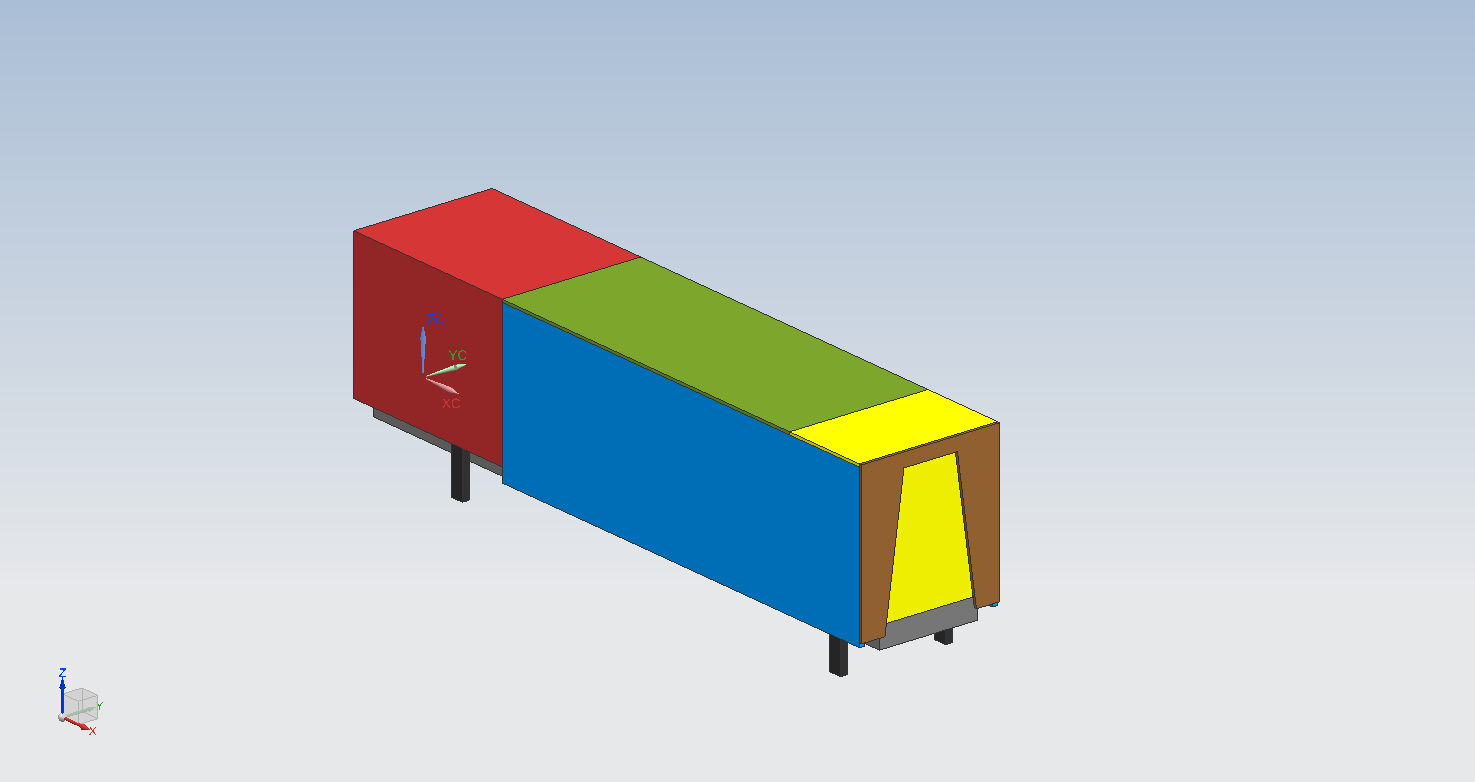
\includegraphics[width=.9\linewidth]{04_figures/B1.png}
      \caption{Modus B1}
      \label{Modus B1}
    \end{subfigure}%
    \begin{subfigure}{.5\textwidth}
      \centering
      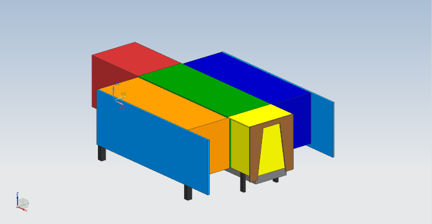
\includegraphics[width=.9\linewidth]{04_figures/B2.png}
      \caption{Modus B2}
      \label{Modus B2}
    \end{subfigure}
  \caption{Modi beim Ausfahren}
\label{Modi beim Ausfahren}
\end{figure}

\paragraph{Wind}
\begin{description}
  \item \textbf{1.1 }
  \item \textbf{1.2 }
\end{description}

\paragraph{Neigung}
Mit Palmer wurde abgesprochen, dass der Boden, auf welchem der Solar Butterfly parkiert wird, die Neigung von 5° (8.8\%) nicht überschreiten darf. Die Implementierung dieser Fälle wird analog zu den Fällen 3.1 - 3.4 im Modus \emph{A} durchgeführt.
\begin{description}
  \item \textbf{2.1 Neigung längs positiv} +5° Neigung des Untergrundes in Fahrtrichtung.
  \item \textbf{2.2 Neigung längs negativ} -5° Neigung des Untergrundes in Fahrtrichtung.
  \item \textbf{2.3 Neigung quer positiv} +5° Neigung des Untergrundes noraml zur Fahrtrichtung. Ansteig befindet sich in Fahrtrichtung rechts.
  \item \textbf{2.4 Neigung quer negativ} -5° Neigung des Untergrundes noraml zur Fahrtrichtung. Ansteig befindet sich in Fahrtrichtung links.
\end{description}

\paragraph{Mobiliar}
\begin{description}
  \item \textbf{3.1 }
  \item \textbf{3.2 }
\end{description}


\subsection{Modus C: Ausgefahren}
Kein einzelner Lastfall für den Wind. Wind ist in den Lastfällen der Panelen enthalten. Die Lasten werden von Yannick und Dominik berechnet:)\\

\begin{center}
  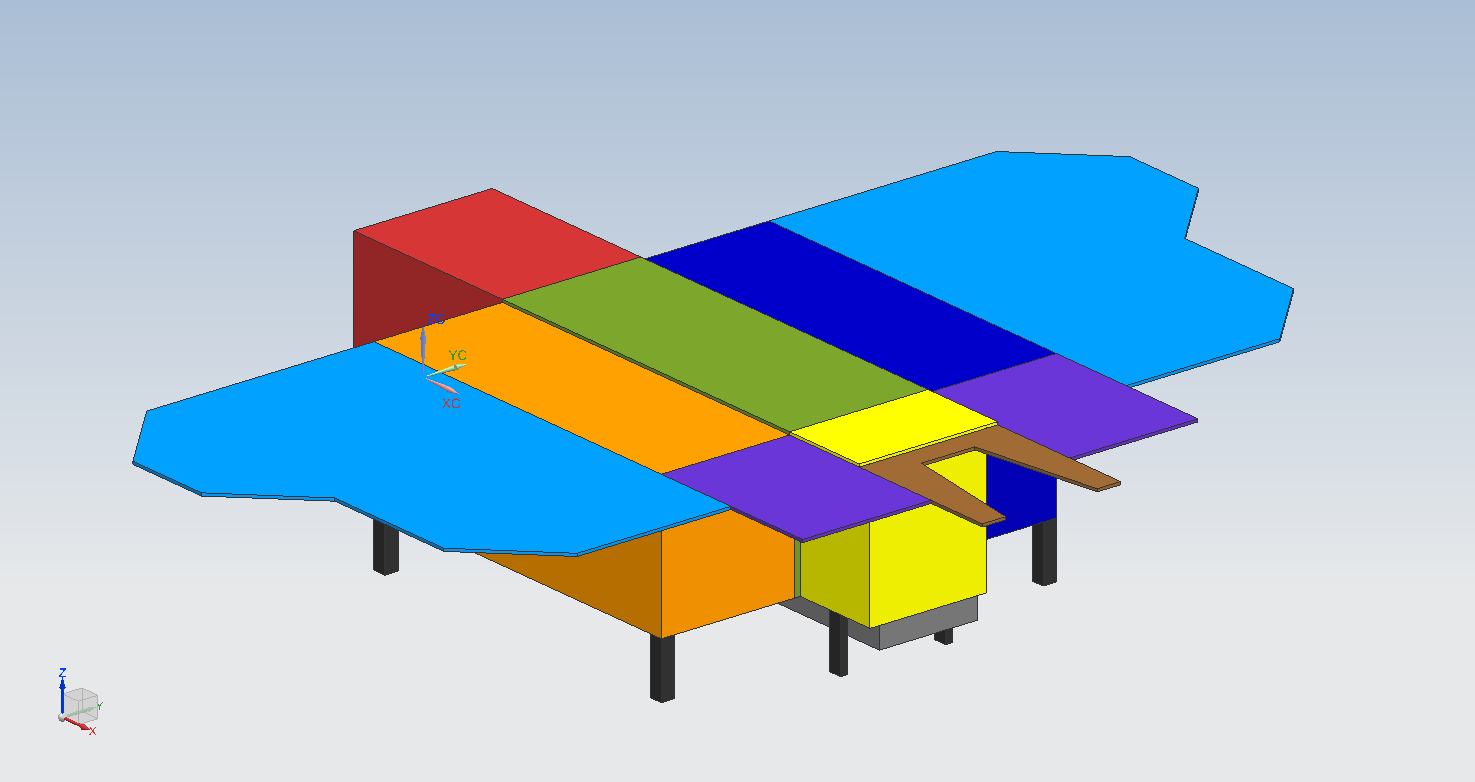
\includegraphics[width=0.5\textwidth]{04_Figures/C.png}
  \captionof{figure}{Modus C}
  \label{Modus C}
\end{center}

\paragraph{Personenlast}
\begin{description}
  \item \textbf{1.1 }
  \item \textbf{1.2 }
\end{description}

\paragraph{Neigung}
Die Lastfälle der Neigung sind analog zum Modus \emph{B}.
\begin{description}
  \item \textbf{2.1 Neigung längs positiv} +5° Neigung des Untergrundes in Fahrtrichtung.
  \item \textbf{2.2 Neigung längs negativ} -5° Neigung des Untergrundes in Fahrtrichtung.
  \item \textbf{2.3 Neigung quer positiv} +5° Neigung des Untergrundes noraml zur Fahrtrichtung. Ansteig befindet sich in Fahrtrichtung rechts.
  \item \textbf{2.4 Neigung quer negativ} -5° Neigung des Untergrundes noraml zur Fahrtrichtung. Ansteig befindet sich in Fahrtrichtung links.
\end{description}

\paragraph{Mobiliar Hauptmodul}
\begin{description}
  \item \textbf{3.1 }
  \item \textbf{3.2 }
\end{description}

\paragraph{Mobiliar Seitenteil}
\begin{description}
  \item \textbf{4.1 }
  \item \textbf{4.2 }
\end{description}

\paragraph{Panelen Klein}
\begin{description}
  \item \textbf{5.1 }
  \item \textbf{5.2 }
\end{description}

\paragraph{Panelen Gross}
\begin{description}
  \item \textbf{6.1 }
  \item \textbf{6.2 }
\end{description}


\subsection{Failuremode}
\paragraph{Temperatur}
\paragraph{Punktlast auf Boden}




\newpage
